\chapter{Transmissão em série de dados HDMI} \label{chap:chap5}

%imp -> https://www.xilinx.com/support/answers/64340.html
Neste capítulo são contempladas todas as arquiteturas desenvolvidas para a transmissão dos dados HDMI em série, explicando todas as decisões tomadas para se obter o produto final. 

\section{Abordagem inicial}

Numa fase inicial do projeto optou-se por abordar de uma maneira simples a transmissão dos dados em série, sem o recurso à definição de todas a tramas do pacote a serem. Tal decisão foi tomada, ciente da importância das tramas num protocolo de comunicação, pois o IP GTX disponibilizado pela \textit{Xilinx} é muito complexo e completo e foi necessário uma familiarização com o mesmo.

\subsection{Transmissão de uma barra de cores gerada na FPGA em série}

A arquitetura desenvolvida in


\subsubsection*{Concepção e Desenvolvimento}
\begin{figure}[h!]
	\begin{center}
		\leavevmode
		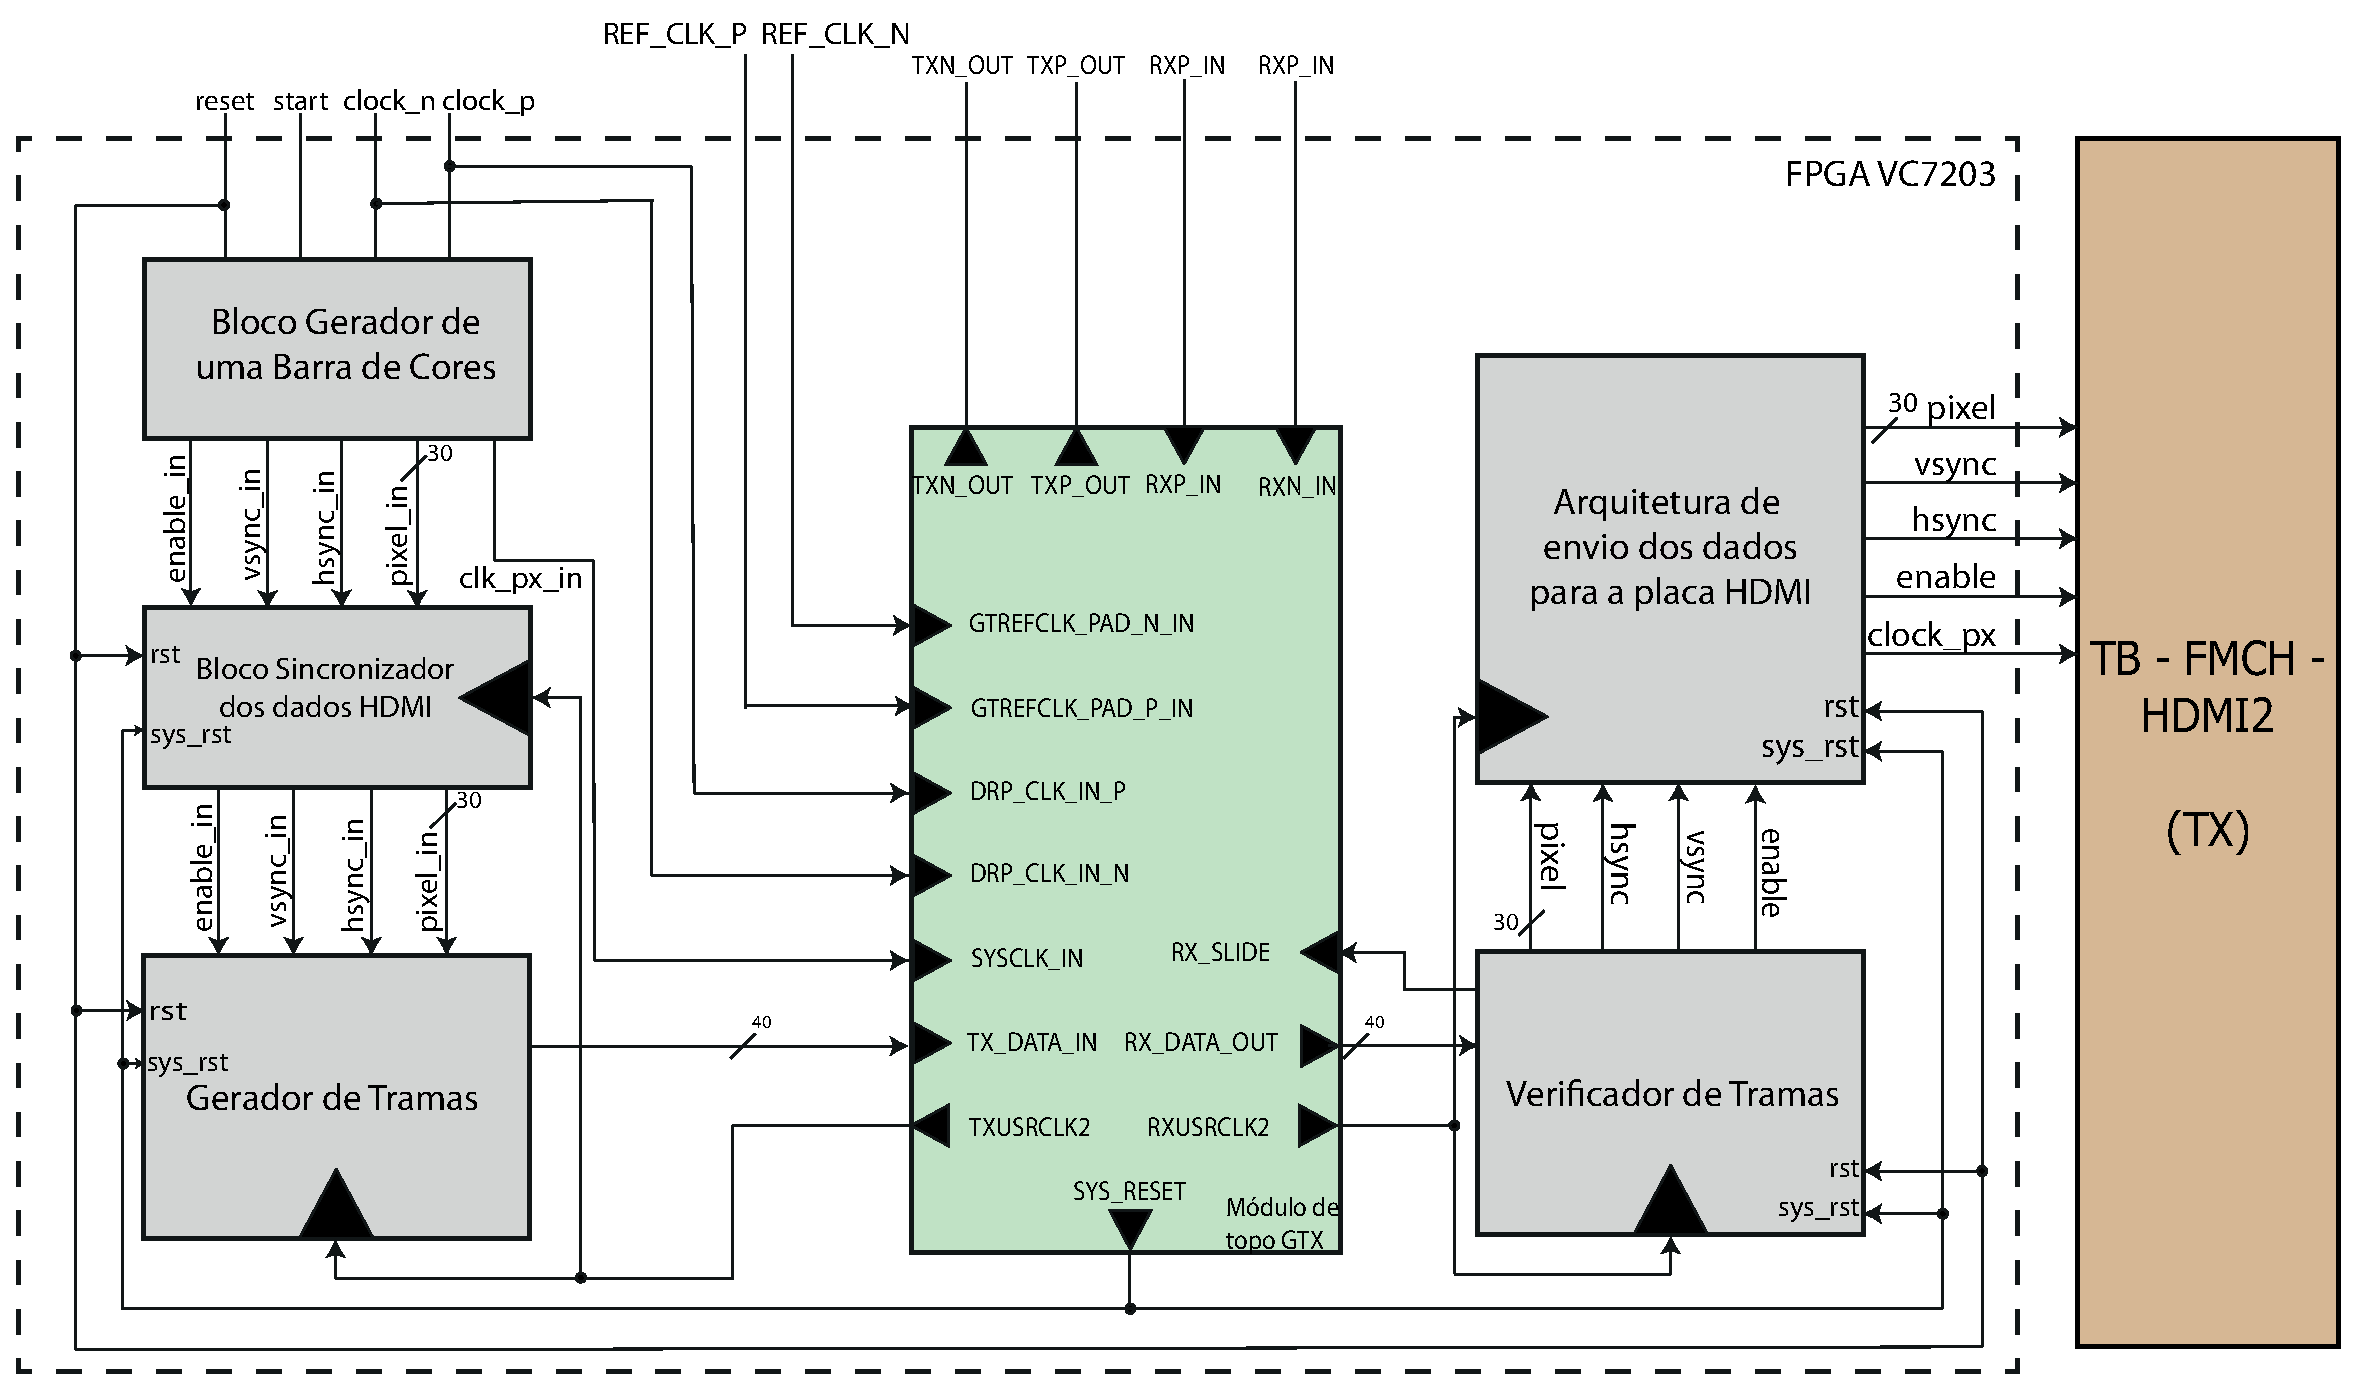
\includegraphics[width=1.0\textwidth]{planod}
		\captionsetup{width=1.0\linewidth}
		\caption[Diagrama de blocos da arquitetura de transmissão em série da barra de cores gerada na FPGA]{Diagrama de blocos da arquitetura de transmissão em série da barra de cores gerada na FPGA}
		\label{fig:planD}
	\end{center}
\end{figure}
\subsubsection*{Resultados}




%\section{Arquiteturas Desenvolvidas}
%
%\subsection{Transmissão em série de uma imagem gerada na FPGA para um dispositivo HDMI de destino}
%
%\subsection{Transmissão em série imagem entre dispositivos HDMI}